\begin{frame}{Funções}

\begin{itemize}
	\item São definidas pela palavra reservada \textit{def}
	\item Podem possuir parâmetros default
	\item São objetos de primeira classe
	\begin{itemize}
		\item Criada em tempo de execução
		\item Pode ser atribuída a uma variável
		\item Passada como argumento para uma função		
		\item Devolvida como resultado de uma função
	\end{itemize}
\end{itemize}
\end{frame}


\begin{frame}{Funções}

\centering \text{Exemplo de função}
\lstset{language=Python}
\lstinputlisting{code/exemplo_funcao.py}
\end{frame}


\begin{frame}{Decoradores }
\begin{center}
	\centering \text{Exemplo de decorador}
	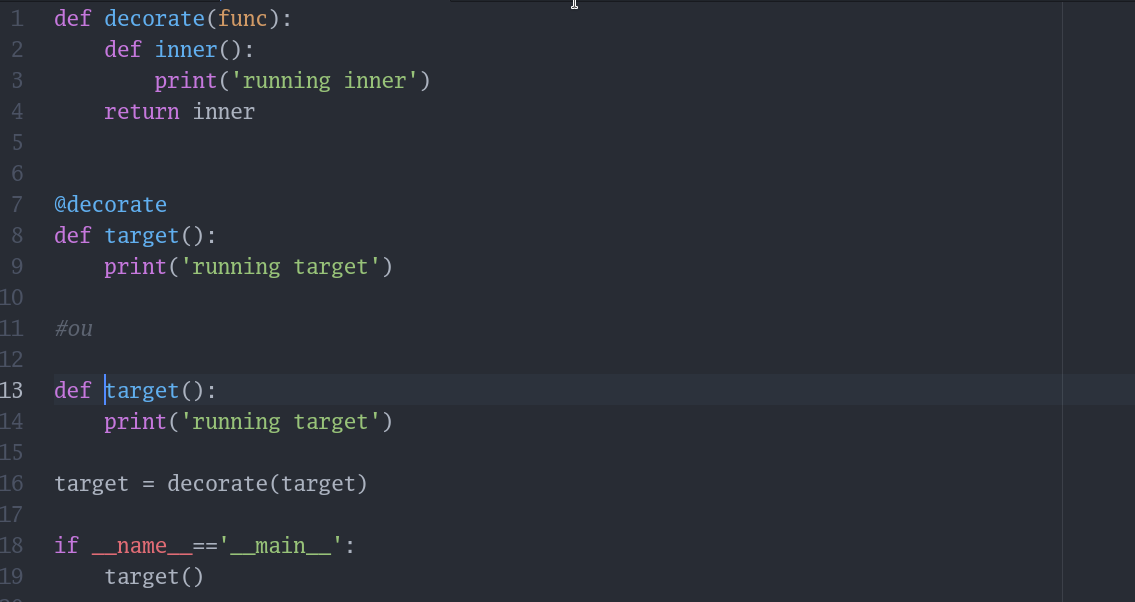
\includegraphics[scale=0.4]{img/decorator_example.png}
\end{center}
\end{frame}

\begin{frame}{Decoradores}

\begin{itemize}
	\item São \textit{callables} que aceitam função como parâmetro 
	\item Criada em tempo de importação
	\item Mudar comportamento de funções ou métodos		
	\item Exemplo real de autenticação no Django
	\item Explícito melhor do que implícito
\end{itemize}

\end{frame}

\begin{frame}{Classes - Classe Carro}

\begin{itemize}
	\item São abstrações de coisas ou comportamentos do mundo real
	\item São definidas com a palavra reservada \textit{class}
	\item Python suporta herança múltipla
	\item Python possui sobrecarga de operadores, assim como C++
	\item Todos os atributos são públicos em Python
	\item Python não possui uma palavra reservada para interface como JAVA, mas o python tem classes abstratas.
	
\end{itemize}

\end{frame}

\begin{frame}{Classes }
\begin{center}
	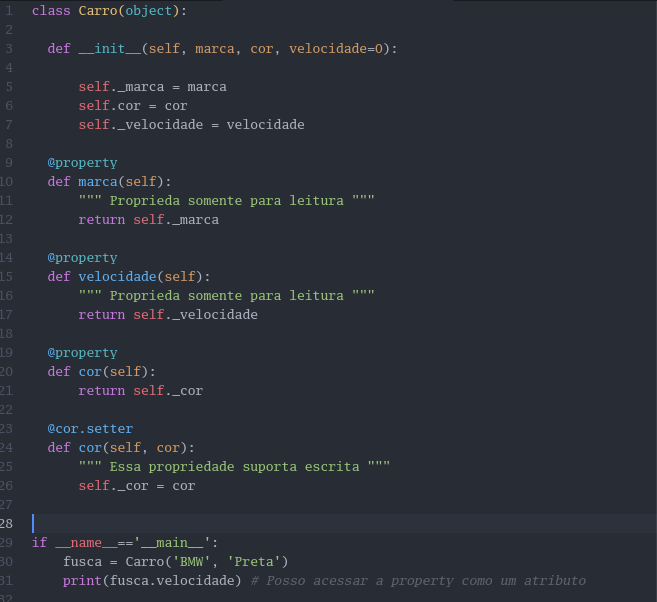
\includegraphics[scale=0.5]{img/class_example.png}
\end{center}
\end{frame}